\graphicspath{{./figures/capitolo6/}}
\lstset{inputpath = ./programs/capitolo6}
\pgfplotstableset{search path = ./tables/capitolo6}

\chapter{Sistemi nonlineari di equazioni}

Nel capitolo precedente abbiamo affrontato lo studio dei sistemi dinamici
lineari e dei loro punti di equilibrio, che nel caso tipico sono unici
e hanno proprietà di stabilità globali
(Teoremi \ref{teor:dinamica-asintotica-lineare-continuo}
e \ref{teor:dinamica-asintotica-lineare-discreto}).
In questo capitolo accenneremo invece al caso nonlineare e ad
alcune condizioni necessarie o sufficienti affinché le dinamiche
siano stabili in un intorno di un punto di equilibrio.
Dopo una breve introduzione teorica, passeremo all'analisi di un
modello matematico per la diagnosi del diabete mellito
e introdurremo il concetto di \emph{stiffness},
che serve a descrivere un certo tipo di difficoltà che si può incontrare
nella soluzione numerica di problemi differenziali dovuta alla presenza
di scale temporali differenti all'interno delle loro soluzioni.

\section{Sistemi nonlineari continui}

Consideriamo il problema di Cauchy nonlineare e non autonomo
\begin{equation} \label{eq:problema-nonlineare-continuo}
\left\{
\begin{aligned}
y'(t)  &= f(t,y(t)) \quad \text{per ogni $t \geq t_0$}, \\
y(t_0) &= y_0 \in \R^m.
\end{aligned}
\right.
\end{equation}
Un punto $\bar{y}$ si dice \emph{punto di equilibrio} o \emph{punto critico}
per l'equazione differenziale $y'(t) = f(t,y(t))$ se $f(t,\bar{y}) = 0$
per ogni $t \geq t_0$, cioè se $y(t) \equiv \bar{y}$ è una soluzione
costante dell'equazione. Dato che qualunque punto di equilibrio $\bar{y}$
può essere traslato nell'origine mediante il cambio di variabile
$z = y - \bar{y}$, per tutto il resto del capitolo lavoreremo sotto
l'ipotesi $\bar{y} = 0$ senza perdere in generalità.
Se la condizione iniziale $y_0$ del problema \eqref{eq:problema-nonlineare-continuo}
è vicina a $\bar{y}$, cosa possiamo dire della traiettoria $y(t)$?
In analogia con il caso lineare, possiamo aspettarci che $y(t)$ sia
attratta da $\bar{y}$, oppure che ne sia respinta, o magari nessuna delle
precedenti. Diamo dunque le seguenti definizioni locali:
\begin{defi}
Senza perdita di generalità, sia $\bar{y} = 0$ un punto di equilibrio
per l'equazione differenziale $y'(t) = f(t,y(t))$. Allora, con riferimento
al problema \eqref{eq:problema-nonlineare-continuo}, la \emph{soluzione nulla}
$y(t) \equiv 0$ si dice
\begin{itemize}
\item \emph{stabile},
	se $\forall \varepsilon > 0$,
	$\forall \tilde{t} \geq t_0$,
	$\exists\, \delta > 0$
	tale che $\norm{y_0} < \delta$
	implica $\norm{y(t,\tilde{t},y_0)} < \varepsilon$
	per ogni $t \geq \tilde{t}$.
	La funzione $t \mapsto y(t,\tilde{t},y_0)$ indica la soluzione del problema
	\eqref{eq:problema-nonlineare-continuo} con condizione iniziale $y(\tilde{t}) = y_0$.
\item \emph{uniformemente stabile},
	se $\forall \varepsilon > 0$,
	$\exists\, \delta > 0$
	tale che $\norm{y_0} < \delta$
	implica $\norm{y(t)} < \varepsilon$
	per ogni $t \geq t_0$.
\item \emph{asintoticamente stabile},
	se è stabile e
	$\exists\, \delta > 0$
	tale che $\norm{y_0} < \delta$
	implica $y(t) \to 0$.
\item \emph{uniformemente asintoticamente stabile},
	se è uniformemente stabile e asintoticamente stabile.
\item \emph{esponenzialmente asintoticamente stabile},
	se $\exists\, \alpha,\beta,\delta > 0$
	tali che $\norm{y_0} < \delta$
	implica $\norm{y(t)} < \alpha \delta e^{-\beta(t-t_0)}$
	per ogni $t \geq t_0$.
\end{itemize}
\end{defi}

\noindent A differenza del caso lineare, in cui molte di queste definizioni
sono equivalenti, nel caso nonlineare è possibile dimostrare tramite degli
esempi che tutte le definizioni sono distinte (e addirittura se ne potrebbero
dare altre, anche se queste sono più che sufficienti per i nostri scopi).
Allo stesso tempo, è chiaro che alcune di queste proprietà di stabilità
ne implicano altre (per esempio, tutte implicano la stabilità semplice).
Vista l'enorme ricchezza e complessità delle dinamiche nonlineari rispetto
al caso lineare, non può esistere una caratterizzazione elementare
di tali proprietà di stabilità in termini di $f(t,y)$ al pari del
Teorema \ref{teor:dinamica-asintotica-lineare-continuo}.
Tuttavia, esistono senz'altro delle condizioni solo necessarie o solo sufficienti
che hanno carattere generale e che possono essere verificate facilmente.
In questo capitolo ne vedremo due: una dovuta al matematico tedesco Oskar Perron,
e una dovuta al matematico russo Aleksandr Mikhailovich Lyapunov.

\subsection*{Linearizzazione e teorema di Perron}

Se $f(t,y)$ è differenziabile rispetto a $y$ nel punto di equilibrio $\bar{y} = 0$,
esiste per definizione un'applicazione lineare $A(t) \in \R^{m \times m}$
detta \emph{matrice jacobiana} tale che
\[
f(t,y) = f(t,0) + A(t)y + g(t,y) = A(t)y + g(t,y),
\quad \text{con $g(t,y) = o(\norm{y})$ per ogni $t \geq t_0$}.
\]
In altre parole, per ogni istante di tempo $t$ fissato, la funzione $y \mapsto f(t,y)$
è ben approssimata nell'origine dalla funzione lineare $y \mapsto A(t)y$,
a meno di infinitesimi superiori al primo.
Pertanto, è ragionevole pensare che nella dinamica del
sistema \eqref{eq:problema-nonlineare-continuo} con valore iniziale
vicino a un punto di equilibrio la componente lineare del moto prenda il
sopravvento su quella non lineare, e che si possano quindi trasferire
risultati di stabilità (o instabilità) dal problema lineare non autonomo
\begin{equation} \label{eq:problema-lineare-nonautonomo-continuo}
\left\{
\begin{aligned}
y'(t)  &= A(t)y(t) \quad \text{per ogni $t \geq t_0$}, \\
y(t_0) &= y_0 \in \R^m
\end{aligned}
\right.
\end{equation}
al problema non lineare \eqref{eq:problema-nonlineare-continuo}.
I seguenti teoremi, di cui non riportiamo la dimostrazione, confermano
che questa intuizione è corretta:

\begin{teor}
Se la soluzione nulla $y(t) \equiv 0$ è uniformemente asintoticamente
stabile per il problema lineare \eqref{eq:problema-lineare-nonautonomo-continuo}
e si ha che
\[
\lim_{y \to 0} \frac{\norm{g(t,y)}}{\norm{y}} = 0
\]
in modo uniforme rispetto a $t$, allora la stessa soluzione nulla
è esponenzialmente asintoticamente stabile per il problema nonlineare
\eqref{eq:problema-nonlineare-continuo}.
\end{teor}

\begin{teor}[Perron] \label{teor:teorema-di-perron-continuo}
Se $A(t) \equiv A$, $\sigma(A) \subseteq \C^-$ e si ha che
\[
\lim_{y \to 0} \frac{\norm{g(t,y)}}{\norm{y}} = 0
\]
in modo uniforme rispetto a $t$, allora la soluzione nulla $y(t) \equiv 0$
è esponenzialmente asintoticamente stabile per il problema nonlineare
\eqref{eq:problema-nonlineare-continuo}. In particolare, nel caso in cui
$A$ e $g(y)$ siano dati dalla linearizzazione di un sistema autonomo,
l'unica ipotesi da verificare è quella sullo spettro di $A$,
cioè la stessa del caso lineare.
\end{teor}

\begin{teor} \label{teor:linearizzazione-instabilità}
Se la soluzione nulla $y(t) \equiv 0$ non è stabile per il problema
\eqref{eq:problema-lineare-nonautonomo-continuo}, allora la stessa soluzione
nulla non può essere stabile nemmeno per il problema nonlineare
\eqref{eq:problema-nonlineare-continuo}.
\end{teor}

\subsection*{Funzioni di Lyapunov}

In meccanica, è ben noto che i punti di minimo locale dell'energia
potenziale sono punti di equilibrio stabili rispetto a piccole
perturbazioni dello stato del sistema. Questa stessa idea
può essere generalizzata al caso di sistemi dinamici nonlineari arbitrari
tramite l'uso delle \emph{funzioni di Lyapunov}, che per semplicità definiamo
nel caso autonomo:

\begin{defi}
Senza perdita di generalità, sia $\bar{y} = 0$ un punto di equilibrio
per l'equazione differenziale $y'(t) = f(t,y(t))$. Una funzione
$V \colon \R^m \to \R$ di regolarità $C^1$ si dice \emph{funzione di Lyapunov}
per tale punto di equilibrio se valgono le seguenti proprietà:
\begin{itemize}
\item $V(y) \geq 0$ per ogni $y \in \R^m$.
\item $V(y) = 0$ se e solo se $y = 0$.
\item $\lim_{\norm{y} \to +\infty} V(y) = +\infty$.
\item Esiste $\delta > 0$ tale che $\norm{y} < \delta$ implica $\grad V(y)^T f(y) \leq 0$.
\item Nell'intorno del punto precedente, si ha che $\grad V(y)^T f(y) = 0$
	se e solo se $y = 0$.
\end{itemize}
\end{defi}

\begin{teor}
Se esiste una funzione di Lyapunov per il punto di equilibrio $\bar{y} = 0$
dell'equazione differenziale $y(t) = f(y(t))$, allora la soluzione nulla
$y(t) \equiv 0$ è asintoticamente stabile per la versione autonoma del
problema \eqref{eq:problema-nonlineare-continuo}.
\end{teor}

\section{Sistemi nonlineari discreti}

Consideriamo il problema ai valori iniziali nonlineare e non autonomo
\begin{equation} \label{eq:problema-nonlineare-discreto}
\left\{
\begin{aligned}
& y_{n+1} = f(n,y_n) \quad \text{per ogni $n \geq n_0$}, \\
& y_{n_0} = y_0 \in \R^m.
\end{aligned}
\right.
\end{equation}
Un punto $\bar{y}$ si dice \emph{punto di equilibrio} o \emph{punto critico}
per l'equazione alle differenze $y_{n+1} = f(n,y_n)$ se $f(n,\bar{y}) = 0$
per ogni $n \geq n_0$, cioè se $y_n \equiv \bar{y}$ è una soluzione
costante dell'equazione. Come nel caso continuo, si può sempre supporre che
$\bar{y} = 0$, e si possono definire analoghe proprietà di stabilità:

\begin{defi}
Senza perdita di generalità, sia $\bar{y} = 0$ un punto di equilibrio
per l'equazione alle differenze $y_{n+1} = f(n,y_n)$. Allora, con riferimento
al problema \eqref{eq:problema-nonlineare-discreto}, la \emph{soluzione nulla}
$y_n \equiv 0$ si dice
\begin{itemize}
\item \emph{stabile},
	se $\forall \varepsilon > 0$,
	$\forall \tilde{n} \geq n_0$,
	$\exists\, \delta > 0$
	tale che $\norm{y_0} < \delta$
	implica $\norm{y(n,\tilde{n},y_0)} < \varepsilon$
	per ogni $n \geq \tilde{n}$.
	La successione $n \mapsto y(n,\tilde{n},y_0)$ indica la soluzione del problema
	\eqref{eq:problema-nonlineare-discreto} con condizione iniziale $y_{\tilde{n}} = y_0$.
\item \emph{uniformemente stabile},
	se $\forall \varepsilon > 0$,
	$\exists\, \delta > 0$
	tale che $\norm{y_0} < \delta$
	implica $\norm{y_n} < \varepsilon$
	per ogni $n \geq n_0$.
\item \emph{asintoticamente stabile},
	se è stabile e
	$\exists\, \delta > 0$
	tale che $\norm{y_0} < \delta$
	implica $y_n \to 0$.
\item \emph{uniformemente asintoticamente stabile},
	se è uniformemente stabile e asintoticamente stabile.
\item \emph{esponenzialmente asintoticamente stabile},
	se $\exists\, \alpha,\delta > 0$,
	$\exists\, \eta \in (0,1)$
	tali che $\norm{y_0} < \delta$
	implica $\norm{y_n} < \alpha \delta \eta^{(n-n_0)}$
	per ogni $n \geq n_0$.
\end{itemize}
\end{defi}

\noindent Se $f(n,y)$ è differenziabile rispetto a $y$ nel punto di equilibrio
$\bar{y} = 0$, l'equazione alle differenze $y_{n+1} = f(n,y_n)$ può essere
linearizzata e si ottiene $y_{n+1} = A_n y_n$.
Anche nel caso discreto si può dimostrare che i risultati di stabilità
(o instabilità) del problema lineare non autonomo
\begin{equation} \label{eq:problema-lineare-nonautonomo-discreto}
\left\{
\begin{aligned}
& y_{n+1} = A_n y_n \quad \text{per ogni $n \geq n_0$}, \\
& y_{n_0} = y_0 \in \R^m
\end{aligned}
\right.
\end{equation}
possono essere trasferiti al problema nonlineare
\eqref{eq:problema-nonlineare-discreto} in un intorno opportuno del punto
di equilibrio:

\begin{teor}
Se la soluzione nulla $y_n \equiv 0$ è uniformemente asintoticamente
stabile per il problema lineare \eqref{eq:problema-lineare-nonautonomo-discreto}
e si ha che
\[
\lim_{y \to 0} \frac{\norm{g(n,y)}}{\norm{y}} = 0
\]
in modo uniforme rispetto a $n$, allora la stessa soluzione nulla
è esponenzialmente asintoticamente stabile per il problema nonlineare
\eqref{eq:problema-nonlineare-discreto}.
\end{teor}

\begin{teor}[Perron]
Se $A_n \equiv A$, $\rho(A) < 1$ e si ha che
\[
\lim_{y \to 0} \frac{\norm{g(n,y)}}{\norm{y}} = 0
\]
in modo uniforme rispetto a $n$, allora la soluzione nulla $y_n \equiv 0$
è esponenzialmente asintoticamente stabile per il problema nonlineare
\eqref{eq:problema-nonlineare-discreto}. In particolare, nel caso in cui
$A$ e $g(y)$ siano dati dalla linearizzazione di un sistema autonomo,
l'unica ipotesi da verificare è quella sullo spettro di $A$,
cioè la stessa del caso lineare.
\end{teor}

\begin{teor}
Se la soluzione nulla $y_n \equiv 0$ non è stabile per il problema
\eqref{eq:problema-lineare-nonautonomo-discreto}, allora la stessa soluzione
nulla non può essere stabile nemmeno per il problema nonlineare
\eqref{eq:problema-nonlineare-discreto}.
\end{teor}

\noindent Vediamo infine come si possa adattare l'approccio basato sulle funzioni
di Lyapunov al caso di sistemi dinamici discreti autonomi:

\begin{defi}
Senza perdita di generalità, sia $\bar{y} = 0$ un punto di equilibrio
per l'equazione alle differenze $y_{n+1} = f(y_n)$. Una funzione
$V \colon \R^m \to \R$ si dice \emph{funzione di Lyapunov}
per tale punto di equilibrio se valgono le seguenti proprietà:
\begin{itemize}
\item $V(y) \geq 0$ per ogni $y \in \R^m$.
\item $V(y) = 0$ se e solo se $y = 0$.
\item $\lim_{\norm{y} \to +\infty} V(y) = +\infty$.
\item Esiste $\delta > 0$ tale che $\norm{y} < \delta$ implica $V(f(y)) \leq V(y)$.
\item Nell'intorno del punto precedente, si ha che $V(f(y)) = V(y)$
	se e solo se $y = 0$.
\end{itemize}
\end{defi}

\begin{teor}
Se esiste una funzione di Lyapunov per il punto di equilibrio $\bar{y} = 0$
dell'equazione alle differenze $y_{n+1} = f(y_n)$, allora la soluzione nulla
$y_n \equiv 0$ è asintoticamente stabile per la versione autonoma del
problema \eqref{eq:problema-nonlineare-discreto}.
\end{teor}

\section{Modello per la diagnosi del diabete mellito}

Il diabete mellito è una malattia che si manifesta sotto forma di
elevata concentrazione di glucosio nel sangue e nelle urine, ed è causata
da una disfunzione del normale meccanismo a retroazione negativa che regola
la concentrazione di glucosio $G(t)$ nel sangue mantenendola intorno
a un valore ottimale $\bar{G}$ anche in seguito a sforzi intensi o all'assunzione
di cibo. La dinamica del livello di glucosio $G(t)$ è molto complessa,
perché influenzata da numerosi processi fisiologici; tra questi la secrezione
di ormoni quali glucagone, adrenalina, cortisolo e insulina.
Quest'ultimo ormone è particolarmente importante perché ha come funzione
quella di favorire l'assorbimento del glucosio da parte delle cellule del nostro
organismo e di conseguenza farne diminuire la concentrazione nel sangue.
Nella pratica clinica non è necessario utilizzare modelli complessi
della dinamica di $G(t)$ per la diagnosi del diabete mellito%
\footnote{Anzi, sarebbe metodologicamente errato utilizzare un modello
con un numero di parametri maggiore al numero di misure che possono essere
realisticamente effettuate su un paziente nel giro di qualche ora.}%
: è sufficiente un modello a due variabili che tenga conto soltanto
della concentrazione di glucosio nel sangue $G(t)$ e dell'ormone insulina $H(t)$.
Supponiamo che a riposo e a digiuno i valori di $G(t)$ e $H(t)$ siano costanti
e pari a dei valori ottimali $\bar{G}$ e~$\bar{H}$. Un test standard per
la diagnosi del diabete mellito noto come \emph{test di tolleranza al glucosio}
prevede la misura a intervalli di tempo regolari (per esempio, mezz'ora)
dei livelli di glucosio nel sangue di un paziente inizialmente a digiuno a cui
sia stata somministrata una quantità standardizzata di acqua e zucchero.
L'analisi del livello basale di glucosio $\bar{G}$ e del tempo necessario affinché
la glicemia ritorni all'equilibrio permettono di formulare una diagnosi di diabete
mellito; in particolare il diabete è diagnosticato per valori di $\bar{G}$
superiori a \SI{126}{mg.dl^{-1}} e per tempi di ritorno all'equilibrio superiori
a 3.5 ore.

Vediamo ora un semplice modello per la dinamica di $G(t)$ e $H(t)$
che possa spiegare i valori della glicemia che si possono osservare
durante un test di tollerenza al glucosio. Supponiamo innanzitutto che tale
dinamica sia indipendente da altri processi fisiologici, e che pertanto si possa
in linea di principio descrivere mediante un sistema di equazioni differenziali
nonlineari autonome:
\[
\left\{
\begin{aligned}
G'(t)  &= F_1(G(t),H(t)) \\
H'(t)  &= F_2(G(t),H(t)).
\end{aligned}
\right.
\]
Nel caso del test di tolleranza al glucosio, stiamo quindi supponendo che
l'aumento del livello di glucosio dovuto all'assorbimento intestinale
si possa concentrare tutto in un unico istante $t=0$.
Se ora linearizziamo questo sistema intorno al punto di equilibrio
$(\bar{G},\bar{H})$ e operiamo il cambio di variabili $g(t) = G(t)-\bar{G}$,
$h(t) = H(t)-\bar{H}$ otteniamo il sistema lineare
\begin{equation} \label{eq:sistema-glucosio-insulina}
\left\{
\begin{aligned}
g'(t)  &= -m_1 g(t) -m_2 h(t) \\
h'(t)  &=  m_3 g(t) -m_4 h(t),
\end{aligned}
\right.
\end{equation}
in cui i segni dei coefficienti sono stati scelti in modo che $m_1,\dots,m_4 > 0$.
Infatti, sia i livelli di glucosio sia i livelli di insulina tendono indipendentemente
a decadere verso i rispettivi livelli basali (segno meno davanti a $m_1$ e $m_4$),
mentre la produzione di insulina è stimolata da un eccesso di glucosio ($+m_3$)
e l'assorbimento di glucosio è promosso da un eccesso di insulina ($-m_2$).
Sia $M$ la matrice associata al sistema lineare \eqref{eq:sistema-glucosio-insulina},
e siano $\lambda_1,\lambda_2 \in \C$ i suoi autovalori. Per il teorema di Perron
\ref{teor:teorema-di-perron-continuo}, ci aspettiamo che $\sigma(M) \subseteq \C^-$,
cosicché si possa dimostrare l'asintotica stabilità della dinamica nonlineare
in un intorno di $(\bar{G},\bar{H})$. In effetti, si può verificare che le
disuguaglianze
\[
\lambda_1 + \lambda_2 = \tr(M) = -m_1-m_4 < 0
\quad \text{e} \quad
\lambda_1 \lambda_2 = \det(M) = m_1 m_4 + m_2 m_3 > 0
\]
sono sufficienti a dimostrare l'inclusione di $\sigma(M)$ in $\C^-$.

Dato che nel test di tolleranza al glucosio il livello di insulina $H(t)$
non viene misurato, conviene derivare rispetto al tempo
la prima equazione del sistema \eqref{eq:sistema-glucosio-insulina} e ricondursi
tramite opportune sostituzioni a un'unica equazione differenziale del
secondo ordine per la dinamica di $g(t)$:
\begin{equation} \label{eq:dinamica-glucosio-alpha-beta}
g''(t) + 2 \alpha g'(t) + \beta^2 g(t) = 0,
\quad \text{con $2 \alpha = m_1 + m_4$ e $\beta^2 = m_1 m_4 + m_2 m_3$}.
\end{equation}
Dal momento che lo smorzamento del livello di glucosio in eccesso $g(t)$ durante
il test di tolleranza al glucosio è solitamente sottocritico, possiamo
supporre che $\Delta = 4(\alpha^2-\beta^2) < 0$ e che quindi la generica
soluzione dell'equazione \eqref{eq:dinamica-glucosio-alpha-beta}
si possa scrivere nella forma
\[
g(t) = A e^{-\alpha t} \sin(\omega t),
\quad \text{con $\omega^2 = \beta^2-\alpha^2 > 0$}.
\]
La fase $\phi$ della funzione seno è stata scelta uguale a zero perché
la prima misura di $G(t)$ in un test di tolleranza al glucosio precede
la somministrazione della dose di glucosio, quindi sappiamo
che $g(0) = 0$. In conclusione, tornando alla variabile originale $G(t)$,
si ha che
\[
G(t) = \bar{G} + A e^{-\alpha t} \sin(\omega t).
\]
I quattro parametri $\bar{G},A,\alpha,\omega$ possono essere stimati a partire
da $n$ misure sperimentali $(t_i,G_i)$ tramite il metodo dei minimi quadrati
nonlineari, cioè andando a minimizzare la funzione
\[
F(\bar{G},A,\alpha,\omega) = \sum_{i=1}^n \bigl(
	G_i - \bar{G} - Ae^{-\alpha t_i} \sin(\omega t_i)
\bigr)^2.
\]
Nella pratica medica, il diabete mellito è diagnosticato quando
$\bar{G} > \SI{126}{mg.dl^{-1}}$ e il semiperiodo $T/2 \deq \pi/\omega$
supera 3.5 ore, cioè si ha un ritorno molto lento al valore di equilibrio
della glicemia (di base più alto rispetto a un individuo non diabetico,
per il quale $\bar{G}$ è solitamente inferiore a \SI{100}{mg.dl^{-1}}).
Gli altri parametri $A$ e $\alpha$ sono invece più sensibili a errori
sperimentali, quindi vengono solitamente ignorati.

Vediamo ora due esempi di come il modello che abbiamo esposto possa essere
applicato a dei dati concreti (di fantasia, ma verosimili).
Nella Figura \ref{fig:paziente-non-diabetico} abbiamo riportato le misure
della glicemia di un paziente non diabetico e la corrispondente curva $G(t)$
ottenuta con il metodo dei minimi quadrati nonlineari.
Abbiamo determinato i seguenti parametri,
\[
\bar{G} = \SI{68.3}{mg.dl^{-1}}, \quad
A = \SI{99.0}{mg.dl^{-1}}, \quad
\alpha = \SI{0.0138}{s^{-1}}, \quad
\omega = \SI{0.0413}{s^{-1}}, \quad
T/2 = \SI{1.27}{\hour},
\]
da cui in effetti non risulta che il paziente sia diabetico.
Nella Figura \ref{fig:paziente-diabetico} abbiamo invece riportato delle misure
di glicemia di un paziente diabetico durante un test di tolleranza al glucosio.
In questo caso il metodo dei minimi quadrati fornisce le seguenti stime:
\[
\bar{G} = \SI{134}{mg.dl^{-1}}, \quad
A = \SI{129}{mg.dl^{-1}}, \quad
\alpha = \SI{0.00798}{s^{-1}}, \quad
\omega = \SI{0.0118}{s^{-1}}, \quad
T/2 = \SI{4.42}{\hour}.
\]
Osserviamo che in effetti $\bar{G} > \SI{126}{mg.dl^{-1}}$ e che
$T/2 > \SI{3.5}{\hour}$, a conferma del fatto che il paziente sia diabetico.
Per quanto riguarda l'aspetto implementativo di questo modello,
abbiamo risolto il problema ai minimi quadrati nonlineari tramite il
comando \code{fit} del \emph{fitting toolbox} di MATLAB,
che internamente utilizza l'algoritmo di Levenberg-Marquardt.
Il codice è riportato nel Programma \ref{prog:diabete}.
Dato che il numero di misure è di poco superiore al numero dei parametri,
è stato importante fornire un valore iniziale ragionevole all'algoritmo
iterativo che risolve il problema ai minimi quadrati.

\begin{figure}[p]
\centering
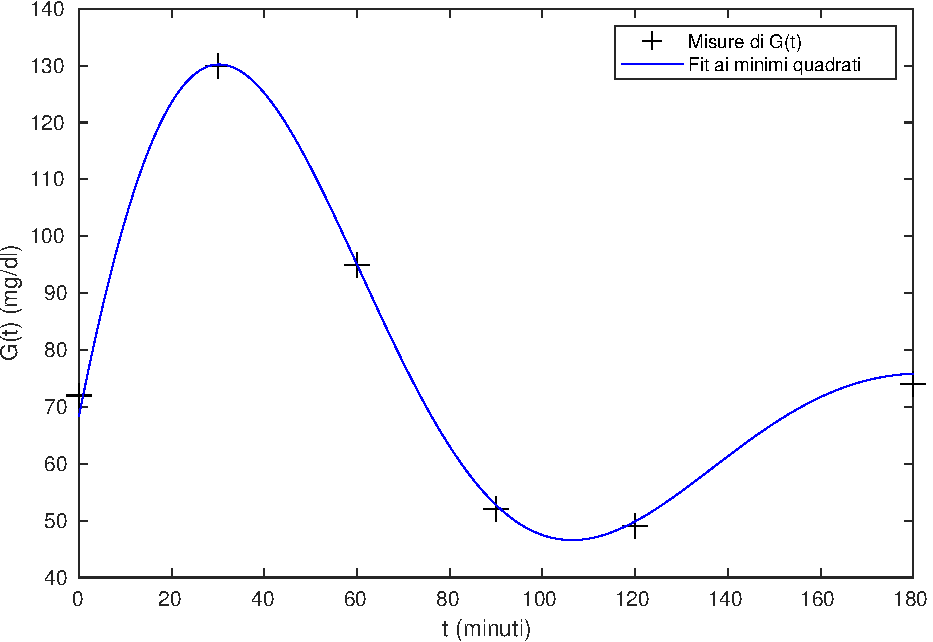
\includegraphics[height=0.27\textheight]{diabete1.pdf}
\caption{Risultati del test di tolleranza al glucosio, paziente non diabetico.}
\label{fig:paziente-non-diabetico}
\end{figure}

\begin{figure}[p]
\centering
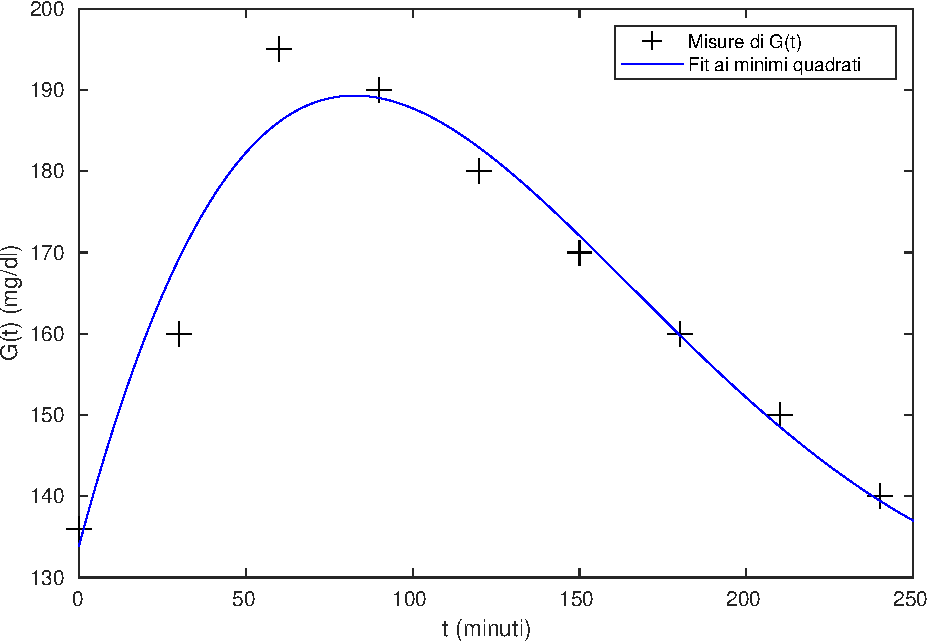
\includegraphics[height=0.27\textheight]{diabete2.pdf}
\caption{Risultati del test di tolleranza al glucosio, paziente diabetico.}
\label{fig:paziente-diabetico}
\end{figure}

\lstinputlisting[float=p, label=prog:diabete, caption={Metodo dei minimi quadrati
nonlineari per la diagnosi del diabete mellito.}]{diabete.m}

\section{Problemi stiff e rapporto di stiffness}

Nel capitolo 3 si è visto come l'uso di metodi numerici espliciti per la soluzione
dell'equazione test $y'(t) = \lambda y(t)$ con $\lambda \ll 0$ e $t \in [0,1]$
sia del tutto inadeguato, nonostante la soluzione $e^{\lambda t} y_0$
sia pressoché costante sul dominio e quindi l'intuito ci suggerisca
che una volta superato il transiente iniziale di ampiezza circa
$\abs{\lambda}^{-1} \ll 1$ si potrebbero adottare senza problemi passi $h$ grandi
(cioè, comparabili con l'ampiezza dell'intervallo temporale di soluzione,
e non con $\abs{\lambda}^{-1}$).
In questo paragrafo andremo a definire una quantità associata a un problema
differenziale, detta \emph{rapporto di stiffness}, che quantifica la difficoltà
riscontrata da certi metodi numerici nella sua soluzione e che generalizza al
caso nonlineare il fenomeno appena descritto per l'equazione test.
Se il rapporto di stiffness è molto maggiore di 1, allora il problema
differenziale è detto \emph{stiff}, e sappiamo che il calcolo numerico della
sua soluzione richiede metodi specifici (per esempio, impliciti).
Per arrivare a definire il rapporto di stiffness nel caso continuo, fissiamo
innanzitutto un problema nonlineare
\begin{equation} \label{eq:problema-nonlineare-continuo-stiffness}
\left\{
\begin{aligned}
y'(t)  &= f(t,y(t)) \quad \text{per ogni $t \in [t_0,T]$}, \\
y(t_0) &= y_0 \in \R^m
\end{aligned}
\right.
\end{equation}
e indichiamo con $y(t,t_0,y_0)$ la sua soluzione, in cui abbiamo messo in evidenza
la dipendenza dall'istante di tempo iniziale $t_0$ e dal valore iniziale $y_0$.
Sia $\eta \in \R^m$ una perturbazione di $y_0$, e definiamo la variazione
$\delta y$ come
\[
\delta y(t,\eta) = y(t,t_0,y_0+\eta) - y(t,t_0,y_0).
\]
Introduciamo ora due quantità, $\kappa$ e $\gamma$, che misurano la variazione
massima e la variazione media sull'intervallo $[t_0,T]$ dovute alla
perturbazione $\eta$ in rapporto alla grandezza della perturbazione stessa:
\[
\kappa(\eta) = \max_{t \in [t_0,T]} \left\lbrace
	\frac{\norm{\delta y(t,\eta)}}{\norm{\eta}} \right\rbrace,
\qquad \gamma(\eta) = \frac{1}{T-t_0} \int_{t_0}^T
	\frac{\norm{\delta y(t,\eta)}}{\norm{\eta}} \dt.
\]
Osserviamo che le quantità $\kappa(\eta)$ e $\gamma(\eta)$ sono ben definite
perché la variazione $\delta y(t,\eta)$ è una funzione continua di $t \in [t0,T]$.
A questo punto, si dice \emph{rapporto di stiffness} del problema
\eqref{eq:problema-nonlineare-continuo-stiffness} il limite
\begin{equation} \label{eq:definizione-rapporto-di-stiffness}
\sigma = \lim_{\delta \to 0^+} \; \sup_{\norm{\eta} \leq \delta} \;
	\frac{\kappa(\eta)}{\gamma(\eta)}.
\end{equation}
Se $\sigma \gg 1$, per esempio $\sigma = 10^5$, allora il problema
\eqref{eq:problema-nonlineare-continuo-stiffness} è detto \emph{stiff}.
Nel caso lineare a coefficienti costanti, cioè $f(t,y) = Ay(t) + b(t)$,
la definizione appena data si semplifica molto grazie alla formula
\eqref{eq:soluzione-problema-lineare-continuo}:
\[
\delta y(t,\eta) = e^{A(t-t_0)} \eta, \quad
\kappa(\eta) = \max_{t \in [t_0,T]} \left\lbrace
	\frac{\norm{e^{A(t-t_0)} \eta}}{\norm{\eta}} \right\rbrace, \quad
\gamma(\eta) = \frac{1}{T-t_0} \int_{t_0}^T
	\frac{\norm{e^{A(t-t_0)} \eta}}{\norm{\eta}} \dt.
\]
Se il problema \eqref{eq:problema-nonlineare-continuo-stiffness} fosse
mal condizionato non avrebbe senso discutere la sua stiffness, quindi
possiamo supporre che tutti gli autovalori $\lambda_i$ di $A$ abbiano
parte reale negativa o nulla. Per semplificare i calcoli, supponiamo
anche che $A$ sia una matrice diagonale (cioè, supponiamo che sia
diagonalizzabile e di aver effettuato un opportuno cambio di variabile). Allora
\[
\norm{e^{A(t-t_0)} \eta} \leq \norm{\eta},
\]
quindi il massimo nella definizione di $\kappa$ è realizzato da $t = t_0$
e si ha $\kappa(\eta) \equiv 1$.
Inoltre, si può dimostrare che la direzione $\eta$ che realizza il $\sup$ nella
definizione di $\sigma$ è quella di un autovettore~$v^-$ relativo a un
autovalore $\lambda^-$ di $A$ con parte reale minima
(cioè $\Re(\lambda^-) \leq \Re(\lambda)$ per ogni $\lambda \in \sigma(A)$).
Si ottiene quindi che
\begin{align*}
\gamma(v^-)
&= \frac{1}{T-t_0} \int_{t_0}^T \frac{\abs{e^{\lambda^-(t-t_0)}} \norm{v^-}}{\norm{v^-}} \dt
 = \frac{1}{T-t_0} \int_{t_0}^T e^{\Re(\lambda^-)(t-t_0)} \dt \\
&= \frac{1}{T-t_0} \left[ \frac{1}{\Re(\lambda^-)} e^{\Re(\lambda^-)(t-t_0)}
	\right]_{t=t_0}^{t=T}
 = \frac{1}{\Re(\lambda^-)(T-t_0)} \left( e^{\Re(\lambda^-)(T-t_0)} - 1 \right).
\end{align*}
Ora, se $e^{\Re(\lambda^-)(T-t_0)} \approx 1$, questo significa che
$\Re(\lambda^-)(T-t_0) \approx 0$ e dalla formula di Taylor per la funzione
esponenziale si ha che $\gamma(v^-) \approx 1$,
quindi $\sigma \approx 1$ e il problema è tutt'altro che stiff.
Se invece $e^{\Re(\lambda^-)(T-t_0)} \approx 0$, si ha che
\[
\gamma(v^-) \approx \frac{1}{\abs{\Re(\lambda^-)}(T-t_0)},
\]
quindi $\sigma \approx \abs{\Re(\lambda^-)}(T-t_0)$.
Se si volesse tenere di conto anche della componente oscillatoria della soluzione,
allora si potrebbe definire il rapporto di stiffness come
\[
\sigma = \abs{\lambdamax}(T-t_0),
\quad \text{con $\abs{\lambdamax}
	= \max_{\lambda_i \in \sigma(A)} \bigl\lbrace \abs{\lambda_i} \bigr\rbrace
	= \rho(A)$}.
\]
Nel caso in cui l'ampiezza dell'intervallo di integrazione $[t_0,T]$ sia scelta
in modo da assicurare il completo smorzamento della componente della soluzione
che decade più lentamente (cioè, il modo associato all'autovalore con parte
reale massima), si ha che $(T-t_0)$ è circa $\abs{\Re(\lambda^+)}^{-1}$,
con $\lambda^+$ autovalore di $A$ con parte reale massima (ovviamente,
questo ragionamento vale solo se $\Re(\lambda^+) \neq 0$). Pertanto,
\[
\sigma \approx \frac{\abs{\Re(\lambda^-)}}{\abs{\Re(\lambda^+)}}.
\]
Nuovamente, se si desidera tenere conto della componente oscillatoria
della soluzione si andrà a definire
$\abs{\lambdamin} = \min \bigl\lbrace \abs{\lambda_i} \bigr\rbrace$
e si avrà quindi
\begin{equation} \label{eq:rapporto-di-stiffness-caso-lineare}
\sigma \approx \frac{\abs{\lambdamax}}{\abs{\lambdamin}}.
\end{equation}
Abbiamo così recuperato una delle definizioni classiche di stiffness
per sistemi di equazioni lineari, a testimonianza della validità della
definizione astratta \eqref{eq:definizione-rapporto-di-stiffness}.
Si noti però il difetto della definizione classica
\eqref{eq:rapporto-di-stiffness-caso-lineare}: non considerando l'intervallo
temporale, individuerebbe come stiff anche un problema in cui
$(T-t_0) \approx \abs{\lambdamax}^{-1}$, che in realtà non è affatto stiff
perché può essere risolto in modo stabile ed efficiente da qualunque metodo
numerico convergente (anche esplicito; basta adottare passi $h$ piccoli).
Al contrario, la definizione \eqref{eq:definizione-rapporto-di-stiffness}
dipende da tutti gli aspetti del problema
\eqref{eq:problema-nonlineare-continuo-stiffness}: l'equazione differenziale
$y'(t) = f(t,y(t))$, la condizione iniziale $y_0$ e l'intervallo di tempo $[t_0,T]$.

Per rendere la definizione \eqref{eq:definizione-rapporto-di-stiffness} più
semplice da calcolare, si può dimostrare che per valori di $\eta$ piccoli
la variazione $\delta y(\tilde{t},\eta)$ è data dalla soluzione al tempo $\tilde{t}$
del sistema lineare non autonomo
\[
\left\{
\begin{aligned}
\delta y'(t)  &= \partial_y f(y(t,t_0,y_0)) \delta y(t)
	\quad \text{per ogni $t \in [t_0,T]$}, \\
\delta y(t_0) &= \eta \in \R^m.
\end{aligned}
\right.
\]
Tuttavia, in molti casi il valore esatto del rapporto di stiffness $\sigma$
rimane impossibile da calcolare per via simbolica (mediante funzioni elementari,
integrali definiti, ecc). Pertanto, spendiamo qualche parola sulla possibilità
di approssimare numericamente il valore $\sigma$. Un approccio in linea
di principio valido, ma computazionalmente molto oneroso, sarebbe quello
di fissare un valore $\delta$ piccolo (tanto nei pressi di 0 la funzione
$\kappa(\eta)/\gamma(\eta)$ è pressoché omogenea) e poi utilizzare un
qualunque algoritmo di ottimizzazione vincolata per determinare il massimo
di $\kappa(\eta)/\gamma(\eta)$ sulla sfera $\norm{\eta} = \delta$.
Dato che nella pratica si verifica quasi sempre che la direzione di $\eta$
che realizza il massimo corrisponda a quella di un autovettore dominante
$v_{\text{max}}$ della matrice jacobiana $\partial_y f(y_0)$, possiamo
saltare il processo di ottimizzazione e calcolare direttamente la stima
\begin{equation} \label{eq:rapporto-di-stiffness-stima}
\sigma \approx \frac{\kappa(v_{\text{max}}\delta)}{\gamma(v_{\text{max}}\delta)},
\quad \text{con $\norm{v_{\text{max}}} = 1$}.
\end{equation}
Osserviamo che, anche se $v_{\text{max}}$ non realizza l'ottimo, questa è comunque
un'utile stima dal basso del vero rapporto di stiffness, il che è sufficiente
in molti casi a dimostrare che un dato problema è stiff.
Abbiamo implementato questa tecnica nel Programma \ref{prog:stiffness-ratio},
che riceve in ingresso i dati che definiscono il problema
\eqref{eq:problema-nonlineare-continuo-stiffness} e fornisce in uscita la
stima di $\sigma$ data dalla formula \eqref{eq:rapporto-di-stiffness-stima}.
In questo caso, per risolvere il problema
\eqref{eq:problema-nonlineare-continuo-stiffness} abbiamo preferito l'uso
del metodo adattativo \code{ode15s} predefinito in MATLAB. Il metodo è
basato sui metodi Runge-Kutta (capitolo 8) ed è indicato per la soluzione
di problemi stiff (suffisso \code{-s}).
Le tolleranze relative e assolute sono state scelte inferiori a $h$,
altrimenti la perturbazione su $y_0$ si confonderebbe con gli
errori dovuti al metodo numerico. Ad ogni modo, non è importante scegliere
tolleranze molto piccole: l'unica cosa che ci interessa di $\sigma$ è il suo
ordine di grandezza, quindi ci bastano una o due cifre significative (su $\sigma$).

\subsection*{Il problema di Van der Pol}

Mettiamo ora a frutto il Programma \ref{prog:stiffness-ratio} per analizzare
la stiffness di un problema concreto. Il seguente problema dipendente
da un parametro $\mu > 0$ è detto \emph{problema di Van der Pol}
\[
\left\{
\begin{aligned}
& y_1'(t) =  y_2(t) \quad \text{per ogni $t \in [0,2\mu]$}, \\
& y_2'(t) = -y_1(t) + \mu y_2(t) (1-y_1(t)^2) \quad \text{per ogni $t \in [0,2\mu]$}, \\
& y_1(0)  = 2, \quad y_2(0) = 0
\end{aligned}
\right.
\]
e le sue soluzioni descrivono un'orbita chiusa attrattiva nel piano $(y_1,y_2)$.
Nella Figura \ref{fig:van-der-pol-stiffness} abbiamo riportato la stima del rapporto
di stiffness $\sigma$ fornita dal Programma \ref{prog:stiffness-ratio} al variare
di $\mu$ da 1 a 1000.
Possiamo osservare che il rapporto di stiffness $\sigma$ è una funzione superlineare
di $\mu$, dunque il problema di Van der Pol è senz'altro stiff per valori $\mu$ grandi.

\lstinputlisting[float=p, label=prog:stiffness-ratio, caption={Stima numerica
del rapporto di stiffness di un problema.}]{stiffness_ratio.m}

\lstinputlisting[float=p, label=prog:dominant-eigenvalue, caption={Approssimazione
grezza di un autovettore dominante di una data matrice.}]{dominant_eigenvalue.m}

\begin{figure}[p]
\centering
\begin{tikzpicture}[trim axis left, trim axis right]
\begin{axis}[
	xlabel={$\mu$},
	ylabel={$\sigma$},
	xmin=-75, xmax=1075, ymax=9e5,
	width=0.9\textwidth,
	height=0.45\textwidth,
]
\addplot[black,mark=*] table[x=mu, y=sigma] {van-der-pol-stiffness.dat};
\end{axis}
\end{tikzpicture}
\caption{Stima del rapporto di stiffness del problema di Van der Pol al variare di $\mu$.}
\label{fig:van-der-pol-stiffness}
\end{figure}

A conferma dell'interpretazione della stiffness come una difficoltà nella soluzione
numerica di un problema, abbiamo riportato nella Figura \ref{fig:van-der-pol-perfratio}
il rapporto $t_e/t_s$ tra il tempo $t_e$ richiesto da un metodo esplicito
come \code{ode23} e il tempo $t_s$ richiesto da un metodo specifico per problemi
stiff come \code{ode23s} per la soluzione del problema di Van der Pol in
funzione del parametro $\mu$.
Le prestazioni dei due metodi sono state misurate per mezzo del
Programma \ref{prog:stiffness-benchmark}.
Ovviamente, al fine di garantire un confronto equo, i due metodi a passo
variabile sono stati eseguiti con la stessa tolleranza sul passo ($10^{-6}$).
Possiamo osservare che, per valori di $\mu$ piccoli, cioè quando il problema non è stiff,
il metodo esplicito è più efficiente, mentre per valori di $\mu$ superiori a 200
il problema di Van der Pol è già sufficientemente stiff da favorire
nettamente il metodo \code{ode23s}. Infine, per $\mu = 1000$, il confronto
è impari: il metodo \code{ode23s} è circa 40 volte più efficiente del metodo \code{ode23}.

\lstinputlisting[float=tbp, label=prog:stiffness-benchmark, caption={Confronto
tra le prestazioni di \code{ode23} e di \code{ode23s} al variare di $\mu$.},
linerange={1-17}]{stiffness_benchmark.m}

\begin{figure}[tbp]
\centering
\begin{tikzpicture}[trim axis left, trim axis right]
\begin{semilogyaxis}[
	xlabel={$\mu$},
	ylabel={$t_e/t_s$},
	xmin=-75, xmax=1075, ymax=80,
	width=0.9\textwidth,
	height=0.5\textwidth,
]
\addplot[black,mark=*] table[x=mu, y=perfratio] {van-der-pol-perfratio.dat};
\addplot[dashed, domain=0:1000] expression {1};
\end{semilogyaxis}
\end{tikzpicture}
\caption{Rapporto tra il tempo di esecuzione richiesto da \code{ode23}
e da \code{ode23s}\\ per il problema di Van der Pol al variare di $\mu$.}
\label{fig:van-der-pol-perfratio}
\end{figure}


























